\documentclass{article}
\usepackage[margin=1in]{geometry}
\usepackage[linesnumbered,ruled,vlined]{algorithm2e}
\usepackage{amsfonts}
\usepackage{amsmath}
\usepackage{amssymb}
\usepackage{amsthm}
\usepackage{enumitem}
\usepackage{fancyhdr}
\usepackage{hyperref}
\usepackage{minted}
\usepackage{multicol}
\usepackage{pdfpages}
\usepackage{standalone}
\usepackage[many]{tcolorbox}
\usepackage{tikz-cd}
\usepackage{transparent}
\usepackage{xcolor}
% \tcbuselibrary{minted}

\author{Nathan Solomon}

\newcommand{\fig}[1]{
    \begin{center}
        \includegraphics[width=\textwidth]{#1}
    \end{center}
}

% Math commands
\renewcommand{\d}{\mathrm{d}}
\DeclareMathOperator{\id}{id}
\DeclareMathOperator{\im}{im}
\DeclareMathOperator{\proj}{proj}
\DeclareMathOperator{\Span}{span}
\DeclareMathOperator{\Tr}{Tr}
\DeclareMathOperator{\tr}{tr}
\DeclareMathOperator{\ad}{ad}
\DeclareMathOperator{\ord}{ord}
%%%%%%%%%%%%%%% \DeclareMathOperator{\sgn}{sgn}
\DeclareMathOperator{\Aut}{Aut}
\DeclareMathOperator{\Inn}{Inn}
\DeclareMathOperator{\Out}{Out}
\DeclareMathOperator{\stab}{stab}

\newcommand{\N}{\ensuremath{\mathbb{N}}}
\newcommand{\Z}{\ensuremath{\mathbb{Z}}}
\newcommand{\Q}{\ensuremath{\mathbb{Q}}}
\newcommand{\R}{\ensuremath{\mathbb{R}}}
\newcommand{\C}{\ensuremath{\mathbb{C}}}
\renewcommand{\H}{\ensuremath{\mathbb{H}}}
\newcommand{\F}{\ensuremath{\mathbb{F}}}

\newcommand{\E}{\ensuremath{\mathbb{E}}}
\renewcommand{\P}{\ensuremath{\mathbb{P}}}

\newcommand{\es}{\ensuremath{\varnothing}}
\newcommand{\inv}{\ensuremath{^{-1}}}
\newcommand{\eps}{\ensuremath{\varepsilon}}
\newcommand{\del}{\ensuremath{\partial}}
\renewcommand{\a}{\ensuremath{\alpha}}

\newcommand{\abs}[1]{\ensuremath{\left\lvert #1 \right\rvert}}
\newcommand{\norm}[1]{\ensuremath{\left\lVert #1\right\rVert}}
\newcommand{\mean}[1]{\ensuremath{\left\langle #1 \right\rangle}}
\newcommand{\floor}[1]{\ensuremath{\left\lfloor #1 \right\rfloor}}
\newcommand{\ceil}[1]{\ensuremath{\left\lceil #1 \right\rceil}}
\newcommand{\bra}[1]{\ensuremath{\left\langle #1 \right\rvert}}
\newcommand{\ket}[1]{\ensuremath{\left\lvert #1 \right\rangle}}
\newcommand{\braket}[2]{\ensuremath{\left.\left\langle #1\right\vert #2 \right\rangle}}

\newcommand{\catname}[1]{{\normalfont\textbf{#1}}}

\newcommand{\up}{\ensuremath{\uparrow}}
\newcommand{\down}{\ensuremath{\downarrow}}

% Custom environments
\newtheorem{thm}{Theorem}[section]

\definecolor{probBackgroundColor}{RGB}{250,240,240}
\definecolor{probAccentColor}{RGB}{140,40,0}
\newenvironment{prob}{
    \stepcounter{thm}
    \begin{tcolorbox}[
        boxrule=1pt,
        sharp corners,
        colback=probBackgroundColor,
        colframe=probAccentColor,
        borderline west={4pt}{0pt}{probAccentColor},
        breakable
    ]
    \color{probAccentColor}\textbf{Problem \thethm.} \color{black}
} {
    \end{tcolorbox}
}

\definecolor{exampleBackgroundColor}{RGB}{212,232,246}
\newenvironment{example}{
    \stepcounter{thm}
    \begin{tcolorbox}[
      boxrule=1pt,
      sharp corners,
      colback=exampleBackgroundColor,
      breakable
    ]
    \textbf{Example \thethm.}
} {
    \end{tcolorbox}
}

\definecolor{propBackgroundColor}{RGB}{255,245,220}
\definecolor{propAccentColor}{RGB}{150,100,0}
\newenvironment{prop}{
    \stepcounter{thm}
    \begin{tcolorbox}[
        boxrule=1pt,
        sharp corners,
        colback=propBackgroundColor,
        colframe=propAccentColor,
        breakable
    ]
    \color{propAccentColor}\textbf{Proposition \thethm. }\color{black}
} {
    \end{tcolorbox}
}

\definecolor{thmBackgroundColor}{RGB}{235,225,245}
\definecolor{thmAccentColor}{RGB}{50,0,100}
\renewenvironment{thm}{
    \stepcounter{thm}
    \begin{tcolorbox}[
        boxrule=1pt,
        sharp corners,
        colback=thmBackgroundColor,
        colframe=thmAccentColor,
        breakable
    ]
    \color{thmAccentColor}\textbf{Theorem \thethm. }\color{black}
} {
    \end{tcolorbox}
}

\definecolor{corBackgroundColor}{RGB}{240,250,250}
\definecolor{corAccentColor}{RGB}{50,100,100}
\newenvironment{cor}{
    \stepcounter{thm}
    \begin{tcolorbox}[
        enhanced,
        boxrule=0pt,
        frame hidden,
        sharp corners,
        colback=corBackgroundColor,
        borderline west={4pt}{0pt}{corAccentColor},
        breakable
    ]
    \color{corAccentColor}\textbf{Corollary \thethm. }\color{black}
} {
    \end{tcolorbox}
}

\definecolor{lemBackgroundColor}{RGB}{255,245,235}
\definecolor{lemAccentColor}{RGB}{250,125,0}
\newenvironment{lem}{
    \stepcounter{thm}
    \begin{tcolorbox}[
        enhanced,
        boxrule=0pt,
        frame hidden,
        sharp corners,
        colback=lemBackgroundColor,
        borderline west={4pt}{0pt}{lemAccentColor},
        breakable
    ]
    \color{lemAccentColor}\textbf{Lemma \thethm. }\color{black}
} {
    \end{tcolorbox}
}

\definecolor{proofBackgroundColor}{RGB}{255,255,255}
\definecolor{proofAccentColor}{RGB}{80,80,80}
\renewenvironment{proof}{
    \begin{tcolorbox}[
        enhanced,
        boxrule=1pt,
        sharp corners,
        colback=proofBackgroundColor,
        colframe=proofAccentColor,
        borderline west={4pt}{0pt}{proofAccentColor},
        breakable
    ]
    \color{proofAccentColor}\emph{\textbf{Proof. }}\color{black}
} {
    \qed \end{tcolorbox}
}

\definecolor{noteBackgroundColor}{RGB}{240,250,240}
\definecolor{noteAccentColor}{RGB}{30,130,30}
\newenvironment{note}{
    \begin{tcolorbox}[
        enhanced,
        boxrule=0pt,
        frame hidden,
        sharp corners,
        colback=noteBackgroundColor,
        borderline west={4pt}{0pt}{noteAccentColor},
        breakable
    ]
    \color{noteAccentColor}\textbf{Note. }\color{black}
} {
    \end{tcolorbox}
}


\fancyhf{}
\setlength{\headheight}{24pt}

\date{\today}
\title{Physics 245 Homework \#1}

\begin{document}
\maketitle

\noindent\fbox{\fbox{\parbox{6.5in}{
    Problem 1.a.
}}}\bigskip\par
Since the given equation doesn't have a phase factor or anything, I will assume that the instantaneous velocity of the string at $t=0$ is zero everywhere. Then we can decompose $y(x,0)$ into a sum of sines and cosines:
\[ y(x,0) = \sum_{n=0}^\infty \left( A_n \sin \left( \frac{n \pi x}{L} \right) + B_n \cos \left( \frac{n \pi x}{L} \right) \right). \]
The differential equation is linear, so we can solve the differential equation term by term, then put the terms back in the sum, to obtain
\[ y(x, t) = \sum_{n=0}^\infty \left( A_n \sin \left( \frac{n \pi x}{L} \right) \cos \left( \frac{n \pi v}{L} t + \varphi  \right) + B_n \cos \left( \frac{n \pi x}{L} \right) \cos \left( \frac{n \pi v}{L} t + \phi \right)  \right). \]
Because we assumed $\frac{\partial}{\partial t} y(x, t) = 0$, the phase factors $\varphi$ and $\phi$ must both be zero. Using our boundary condition that $y(0, t)=0$ for all $t$, we also see that every $B_n$ must be zero. Lastly, $A_0$ may as well be zero because $\sin(0)=0$. Now the equation can be simplified to
\[ y(x, t) = \sum_{n=1}^\infty A_n \sin \left( \frac{n \pi x}{L} \right) \cos \left( \frac{n \pi v}{L} t \right). \]

\bigskip
\noindent\fbox{\fbox{\parbox{6.5in}{
    Problem 1.b.
}}}\bigskip\par
The coefficients $A_n$ are given by the Fourier transform, which we can evaluate using integration by parts.
\begin{align*}
    A_n &= \frac{2}{L} \int_{x=0}^L \sin \left( \frac{n \pi x}{L} \right) y(x, 0) \d x \\
        &= \frac{2}{L} \int_{x=0}^{L/2} \sin \left( \frac{n \pi x}{L} \right) \frac{2xd}{L} \d x + \frac{2}{L} \int_{x=L/2}^L \sin \left( \frac{n \pi x}{L} \right) \frac{2d(L-x)}{L} \d x \\
        &= \frac{2}{L} \left( \left[ \frac{2xd}{L} \cdot \left( - \frac{L}{n \pi} \cos \left( \frac{n \pi x}{L} \right) \right) \right]_{x=0}^{L/2} - \int_{x=0}^{L/2} \frac{2d}{L} \cdot \left( - \frac{L}{n \pi} \cos \left( \frac{n \pi x}{L} \right) \right) \d x \right)  + \frac{2}{L} \int_{x=L/2}^L \sin \left( \frac{n \pi x}{L} \right) \frac{2d(L-x)}{L} \d x \\
        &= \frac{4d}{Ln \pi} \left( \left[ -x \cos \left( \frac{n \pi x}{L} \right) \right]_{x=0}^{L/2} + \left[ \frac{L}{n\pi} \sin \left( \frac{n \pi x}{L} \right) \right]_{x=0}^{L/2} \right)  + \frac{2}{L} \int_{x=L/2}^L \sin \left( \frac{n \pi x}{L} \right) \frac{2d(L-x)}{L} \d x \\
        &= \frac{4d}{Ln \pi} \left( \frac{L}{2} \cos \left( \frac{n\pi}{2} \right) + \frac{L}{n\pi} \sin \left( \frac{n \pi}{2} \right) \right) + \frac{4d}{L} \int_{x=L/2}^L \sin \left( \frac{n \pi x}{L} \right) \d x - \frac{4d}{L^2} \int_{x=L/2}^L x \sin \left( \frac{n \pi x}{L} \right) \d x  \\
        &= \frac{4d}{Ln \pi} \left( \frac{L}{2} \cos \left( \frac{n\pi}{2} \right) + \frac{L}{n\pi} \sin \left( \frac{n \pi}{2} \right) \right) + \frac{4d}{L} \left[ - \frac{L}{n \pi} \cos \left( \frac{n \pi x}{L} \right) \right]_{x=L/2}^L - \frac{4d}{L^2} \int_{x=L/2}^L x \sin \left( \frac{n \pi x}{L} \right)  \d x \\
        &= \frac{4d}{Ln \pi} \left( \frac{L}{2} \cos \left( \frac{n\pi}{2} \right) + \frac{L}{n\pi} \sin \left( \frac{n \pi}{2} \right) - L \cos \left( n \pi \right) + L \cos \left( \frac{n\pi}{2} \right) \right) - \frac{4d}{L^2} \int_{x=L/2}^L x \sin \left( \frac{n \pi x}{L} \right) \d x  \\
        &= \frac{4d}{Ln \pi} \left( \frac{L}{2} \cos \left( \frac{n\pi}{2} \right) + \frac{L}{n\pi} \sin \left( \frac{n \pi}{2} \right) - L (-1)^n \right) + \frac{4d}{L^2} \left( \left[ x \frac{L}{n\pi} \cos \left( \frac{n \pi x}{L} \right) \right]_{x=L/2}^L + \int_{x=L/2}^L \left( - \frac{L}{n\pi} \cos \left( \frac{n \pi x}{L} \right) \right) \d x\right)  \\
        &= \frac{4d}{Ln \pi} \left( \frac{L}{2} \cos \left( \frac{n\pi}{2} \right) + \frac{L}{n\pi} \sin \left( \frac{n \pi}{2} \right) - L (-1)^n + \left[ x \cos \left( \frac{n \pi x}{L} \right) \right]_{x=L/2}^L + \int_{x=L/2}^L \left( - \cos \left( \frac{n \pi x}{L} \right) \right) \d x\right)  \\
        &= \frac{4d}{Ln \pi} \left( \frac{L}{2} \cos \left( \frac{n\pi}{2} \right) + \frac{L}{n\pi} \sin \left( \frac{n \pi}{2} \right) - L (-1)^n + L(-1)^n - \frac{L}{2} \cos \left( \frac{n \pi}{2} \right) + \left[- \frac{L}{n\pi} \sin \left( \frac{n \pi x}{L} \right) \right]_{x=L/2}^L \right) \\
        &= \frac{4d}{Ln \pi} \cdot \frac{2L}{n\pi} \sin \left( \frac{n \pi}{2} \right) \\
        &= \frac{8d}{n^2 \pi^2} \sin \left( \frac{n \pi}{2} \right) \\
\end{align*}
Therefore the first nonzero coefficients are
\begin{align*}
    A_1 &= \frac{8d}{\pi^2} \\
    A_3 &= - \frac{8d}{9 \pi^2} \\
    A_5 &= \frac{8d}{25 \pi^2}
\end{align*}

\bigskip
\noindent\fbox{\fbox{\parbox{6.5in}{
    Problem 1.c.
}}}\bigskip\par
The differential equation is linear, so each vibrational mode will not affect other vibrational modes. That means if we approximate the formula given in part (a) with a partial sum, that approximation will be just as valid at a later time.

\bigskip
\noindent\fbox{\fbox{\parbox{6.5in}{
    Problem 3.a.
}}}\bigskip\par
\begin{align*}
    M &= \frac{\Omega}{4i\hbar} \sigma_x \\
    \exp(Mt) &= \sum_{n=0}^\infty \frac{1}{n!} (Mt)^n \\
             &= \left( I_2 + \frac{M^2t^2}{2!} + \frac{M^4t^4}{4!} + \cdots \right) + \left( Mt + \frac{M^3t^3}{3!} + \frac{M^5t^5}{5!} + \cdots \right) \\
             &= \left( \sum_{n=0}^\infty \frac{1}{(2n)!} \left( \frac{\Omega t}{4 i \hbar} \right)^{2n} \right) I_2 + \left( \sum_{n=0}^\infty \frac{1}{(2n+1)!} \left( \frac{\Omega t}{4 i \hbar} \right)^{2n+1} \right) \sigma_x \\
             &= \left( \sum_{n=0}^\infty \frac{(-1)^n}{(2n)!} \left( \frac{\Omega t}{4 \hbar} \right)^{2n} \right) I_2 - \left( \sum_{n=0}^\infty \frac{(-1)^n}{(2n+1)!} \left( \frac{\Omega t}{4 \hbar} \right)^{2n+1} \right) i \sigma_x \\
             &= \cos \left( \frac{\Omega}{4 \hbar} t \right) I_2 - i \sin \left( \frac{\Omega}{4 \hbar} t \right) \sigma_x \\
             &= \begin{bmatrix}
                 \cos \left( \frac{\Omega}{4 \hbar} t \right) & - i \sin \left( \frac{\Omega}{4 \hbar} t \right) \\
                 - i \sin \left( \frac{\Omega}{4 \hbar} t \right) & \cos \left( \frac{\Omega}{4 \hbar} t \right)
             \end{bmatrix}
\end{align*}
If we suppose that initially, $a_1=1$ and $a_2=0$, then the state after time $t$ is the first column of $\exp(Mt)$. Otherwise, the state after time $t$ is the initial state left-multiplied by $\exp(Mt)$.

\bigskip
\noindent\fbox{\fbox{\parbox{6.5in}{
    Problem 4.a.
}}}\bigskip\par
The spatial function for the $n$th state is given by
\[ \Psi_n = \sqrt{ \frac{2}{L}} \sin \left( \frac{n\pi x}{L} \right), 0 \leq x \leq L. \]
Since this function has reflectional symmetry (about $x = L/2$), the expected value $\mean{x}$ must be $L/2$, and $\mean{p}$ must be zero.

\bigskip
\noindent\fbox{\fbox{\parbox{6.5in}{
    Problem 4.b.
}}}\bigskip\par
\begin{align*}
    \sigma_x^2 &= \mean{x^2} - \mean{x}^2 \\
               &= \left( \int_{x=0}^L \Psi_n^* x^2 \Psi_n \d x  \right) - \frac{L^2}{4} \\
               &= \left( \frac{2}{L} \int_{x=0}^L x^2 \sin^2 \left( \frac{n \pi x}{L} \right)  \d x  \right) - \frac{L^2}{4} \\
               &= \left( \frac{L^2}{3} - \frac{L^2}{2 n^2 \pi^2} \right)  - \frac{L^2}{4} \\
               &= \frac{L^2}{12} - \frac{L^2}{2 n^2 \pi^2} \\
    \sigma_x = \sqrt{\sigma_x^2} &= L \sqrt{\frac{1}{12} - \frac{1}{2 n^2 \pi^2}} \\
    \sigma_p^2 &= \int_{x=0}^L \Psi_n^* (p-\mean{p})^2 \Psi_n \d x \\
               &= \frac{2}{L} \int_{x=0}^L \sin \left( \frac{n \pi x}{L} \right) \left( -\hbar^2 \frac{\partial^2}{\partial x} \right) \sin \left( \frac{n \pi x}{L} \right) \d x \\
               &= \frac{2n^2\pi^2\hbar^2}{L^3} \int_{x=0}^L \sin^2 \left( \frac{n \pi x}{L} \right) \d x \\
               &= \frac{n^2\pi^2\hbar^2}{L^2} \\
    \sigma_p = \sqrt{\sigma_p^2} &= \frac{n\pi \hbar}{L}
\end{align*}
These answers are reasonable because they satisfy the Heisenberg uncertainty principle, and because $\sigma_x$ and $\sigma_p$ both increase as $n$ increases.
\begin{align*}
    \sigma_x \sigma_p &= n \pi \hbar \sqrt{ \frac{1}{12} - \frac{1}{2 n^2 \pi^2}} \\
                      &\geq \pi \hbar \sqrt{ \frac{1}{12} - \frac{1}{2 \pi^2}} \geq \hbar \sqrt{ \frac{\pi^2}{12} - \frac{1}{2}} \geq \hbar \sqrt{ \frac{9-6}{12}} \geq \frac{\hbar}{2}.
\end{align*}

\bigskip
\noindent\fbox{\fbox{\parbox{6.5in}{
    Problem 5.a.
}}}\bigskip\par
This state, $\ket{s= \frac{1}{2}, m_s = \frac{1}{2}}$, is an eigenstate of $S^2$ (with eigenvalue $\hbar^2 s (s+1)$) and an eigenstate of $S_z$ (with eigenvalue $\hbar m_s = \frac{\hbar}{2}$). Therefore, the uncertainties in $S^2$ and in $S_z$ are both zero. Since $\ket{\Psi_1} = \begin{bmatrix}
    1 \\
    0
\end{bmatrix} = \frac{1}{\sqrt{2}} \ket{+X} - \frac{1}{\sqrt{2}} \ket{-X}$, where $\ket{+X} = \frac{1}{\sqrt{2}} \begin{bmatrix}
    1 \\
    1
\end{bmatrix}$ and $\ket{-X} = \frac{1}{\sqrt{2}}\begin{bmatrix}
    1 \\
    -1
\end{bmatrix}$ are the eigenvectors of $S_x$, $S_x$ has a one half chance of being measured as $\frac{\hbar}{2}$ (the eigenvalue of $\ket{+X}$) and a one half chance of being $-\frac{\hbar}{2}$ (the eigenvalue of $\ket{-X}$), so the uncertainty in $S_x$ is $\frac{\hbar}{2}$.

\bigskip
\noindent\fbox{\fbox{\parbox{6.5in}{
    Problem 5.b.
}}}\bigskip\par
By the same logic as in part (a), the uncertainty in $S^2$ and in $S_x$ are zero, but since $S_z$ has a half chance each of being measured as positive and negative $\frac{\hbar}{2}$, the uncertainty in $S_z$ is $\frac{\hbar}{2}$.
\bigskip
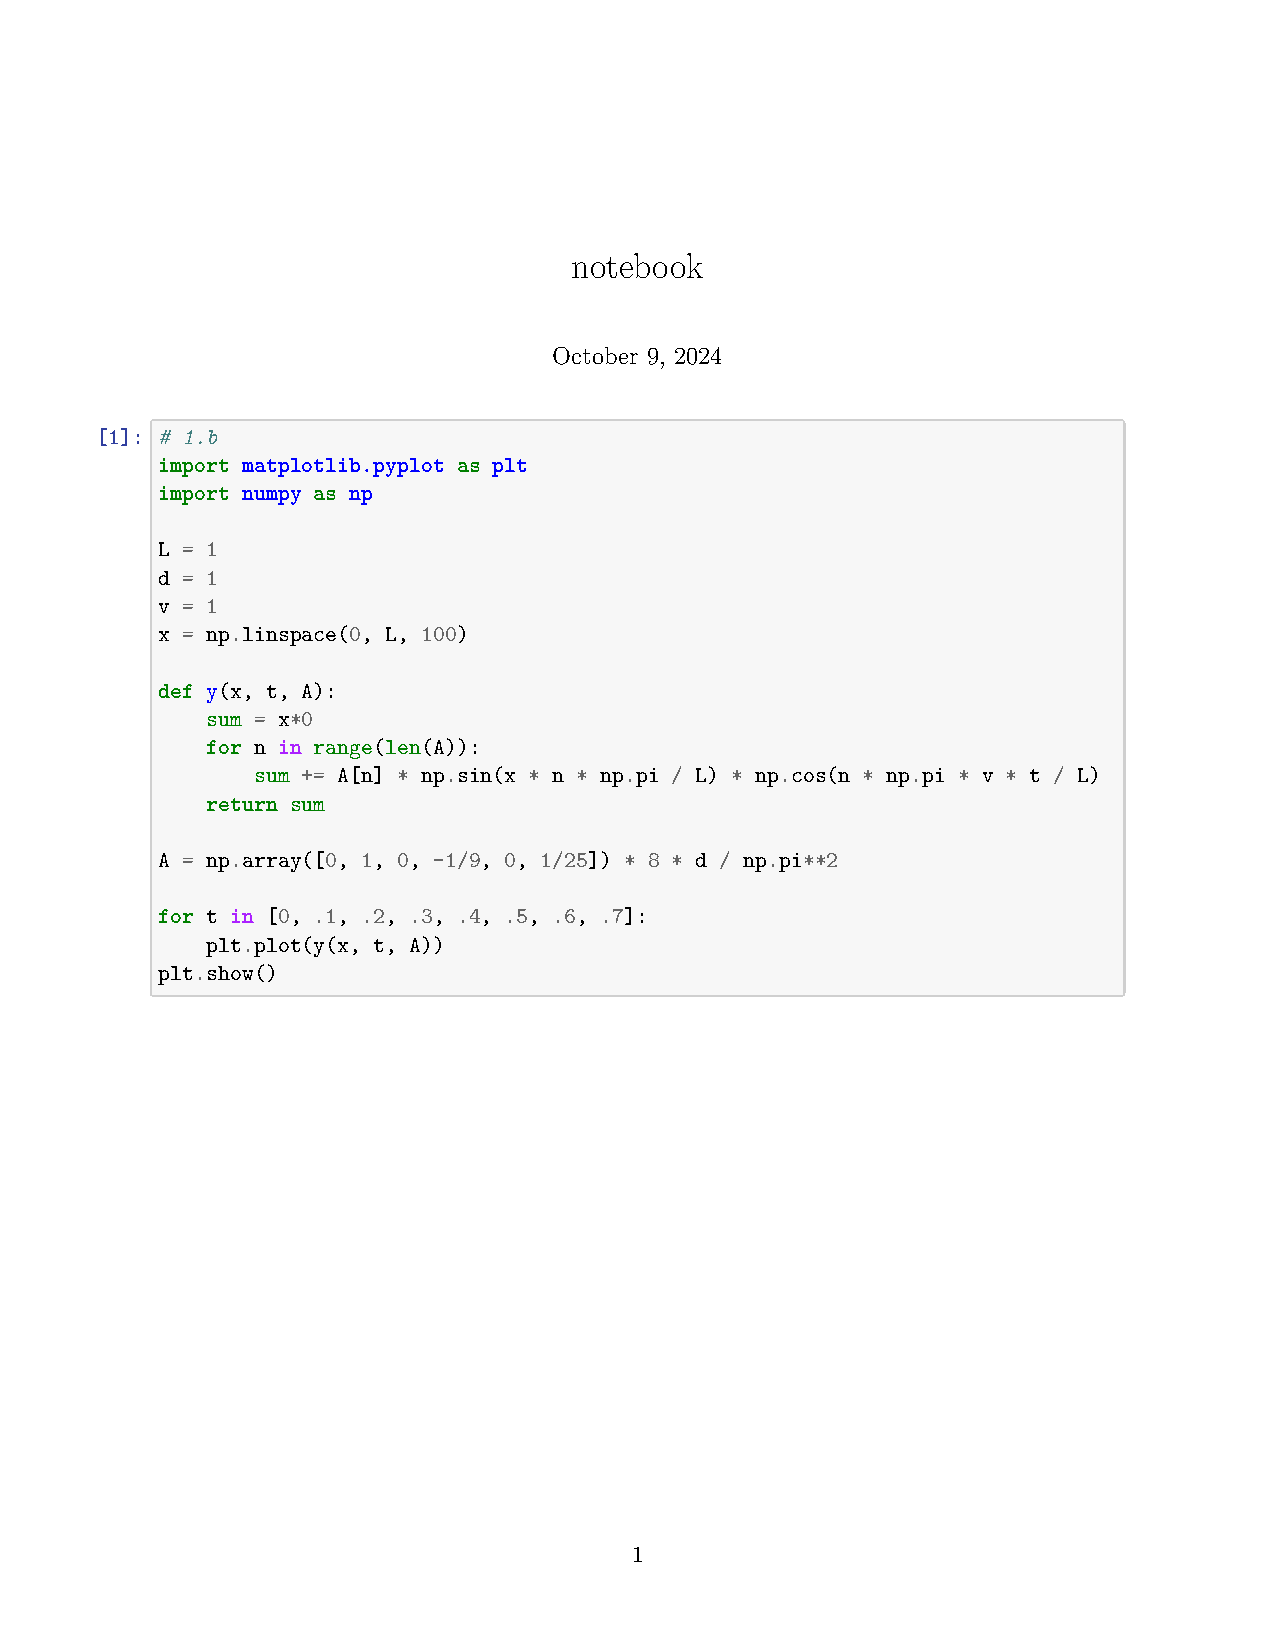
\includepdf[pages=-]{notebook.pdf}
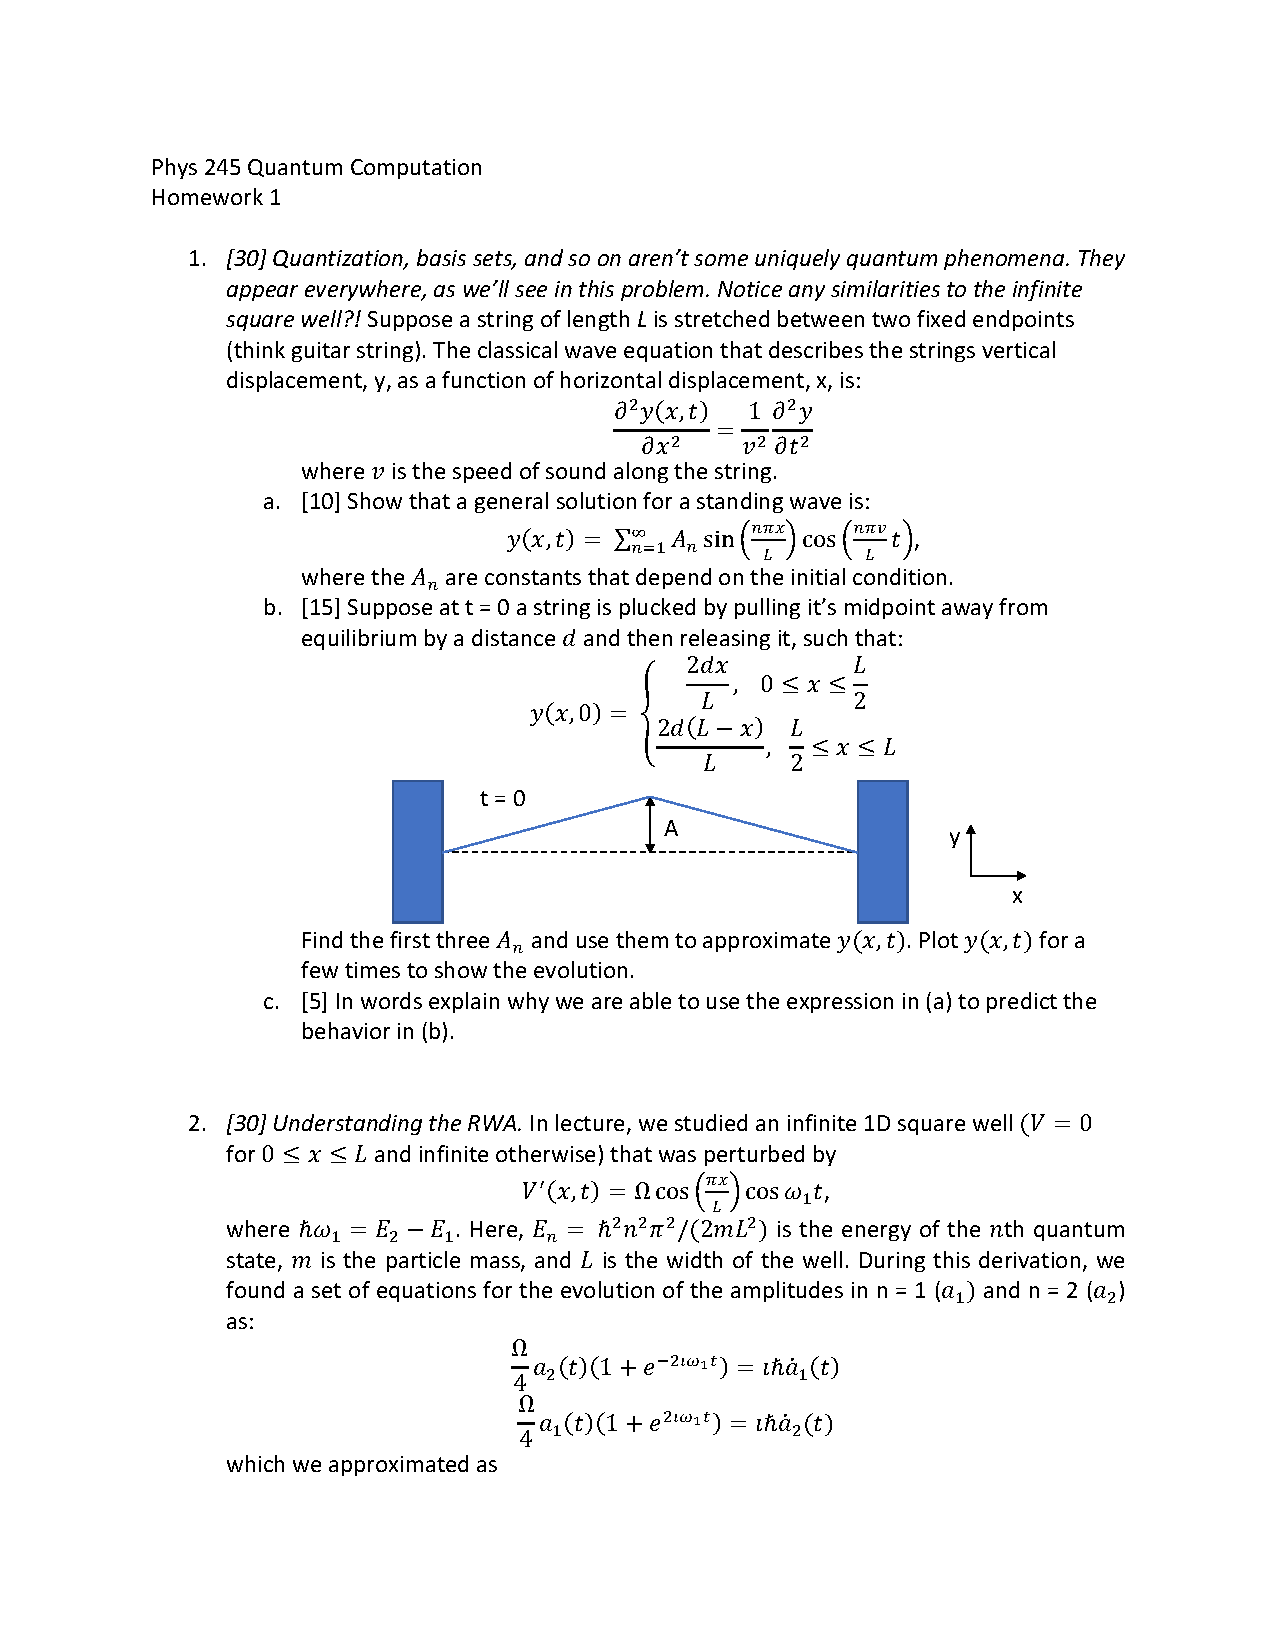
\includepdf[pages=-]{assignment.pdf}

\end{document}
